%# -*- coding: utf-8-unix -*-
%%==================================================
\chapter{文字识别(Scene Text Recognition)}
近期的文字识别的文章主要围绕两个主题进行展开:1)如何得到更准的对齐的字符特征;2)如何高效地利用文本的语义特征进行识别。

DAN\cite{wang2019decoupled},GTC\cite{hu2020gtc}以及TextScanner\cite{wan2019textscanner}都是针对第一个问题进行改进。DAN认为注意力模型中
因需要依赖前一时刻预测结果从而存在累积误差使得模型的attention难以对齐,文中通过解耦注意力模块和文本语义预测模块使得attention更为准确。
GTC认为基于CTC的文本识别器中,因为CTC的切割使得特征难以对齐。文中通过注意力模块来指导CTC的训练,从而使得特征在一定程度对齐。
TextScanner通过预测字符的阅读顺序从而缓解字符定位问题。

SCATTER\cite{scatter}和SRN\cite{2020srn}都是针对第二个问题进行改进。SCATTER通过在视觉特征和语义特征之间迭代地使用注意力机制从而动态选择视觉和语义特征来加强分类效果。
SRN通过并行化注意力模块和语义模块,使得当前帧在预测时能够获得前向和后向的所有视觉以及语义特征,从而加强分类效果。
\section{文字识别方法介绍}
\subsection{DAN (AAAI2020)}
DAN\cite{wang2019decoupled}的主要是解决基于attention机制的识别器中因需要依赖先前预测结果(存在错误累积)所导致的注意力不对齐的问题。
文章中通过解耦注意力机制和语义模型来解决该问题。解耦过程如图\ref{dan_introduction}所示。
\begin{figure}[H]
    \centering
    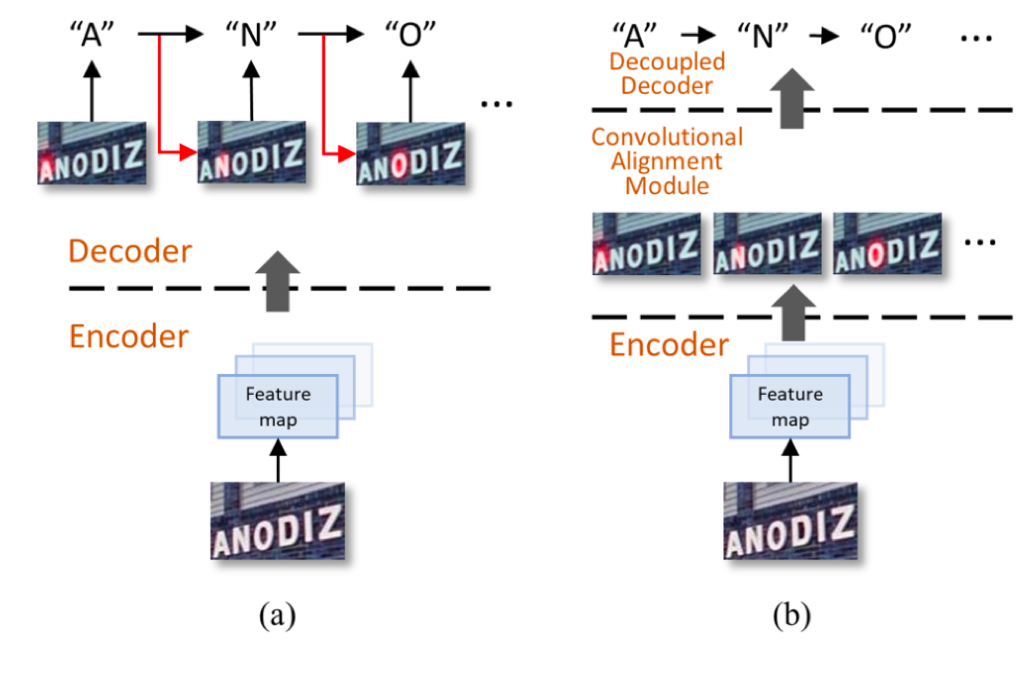
\includegraphics[width=.6\textwidth]{figure/recognition/dan_introduction.png} 
    \caption{DAN解耦过程:(a)之前的基于注意力机制的方法将注意力模块和语义推理模块放在一起;(b)DAN
    中先预测注意力,然后进行语义模块的预测。} 
    \label{dan_introduction} 
\end{figure}

\subsubsection{DAN的网络结构}
DAN的网络结构如图\ref{dan_framework}所示:Decoupled Text Decoder是基于GRU的,其过程和其他文字识别器的一致;
CAM用于预测每一步的attention map。
\begin{figure}[H]
    \centering
    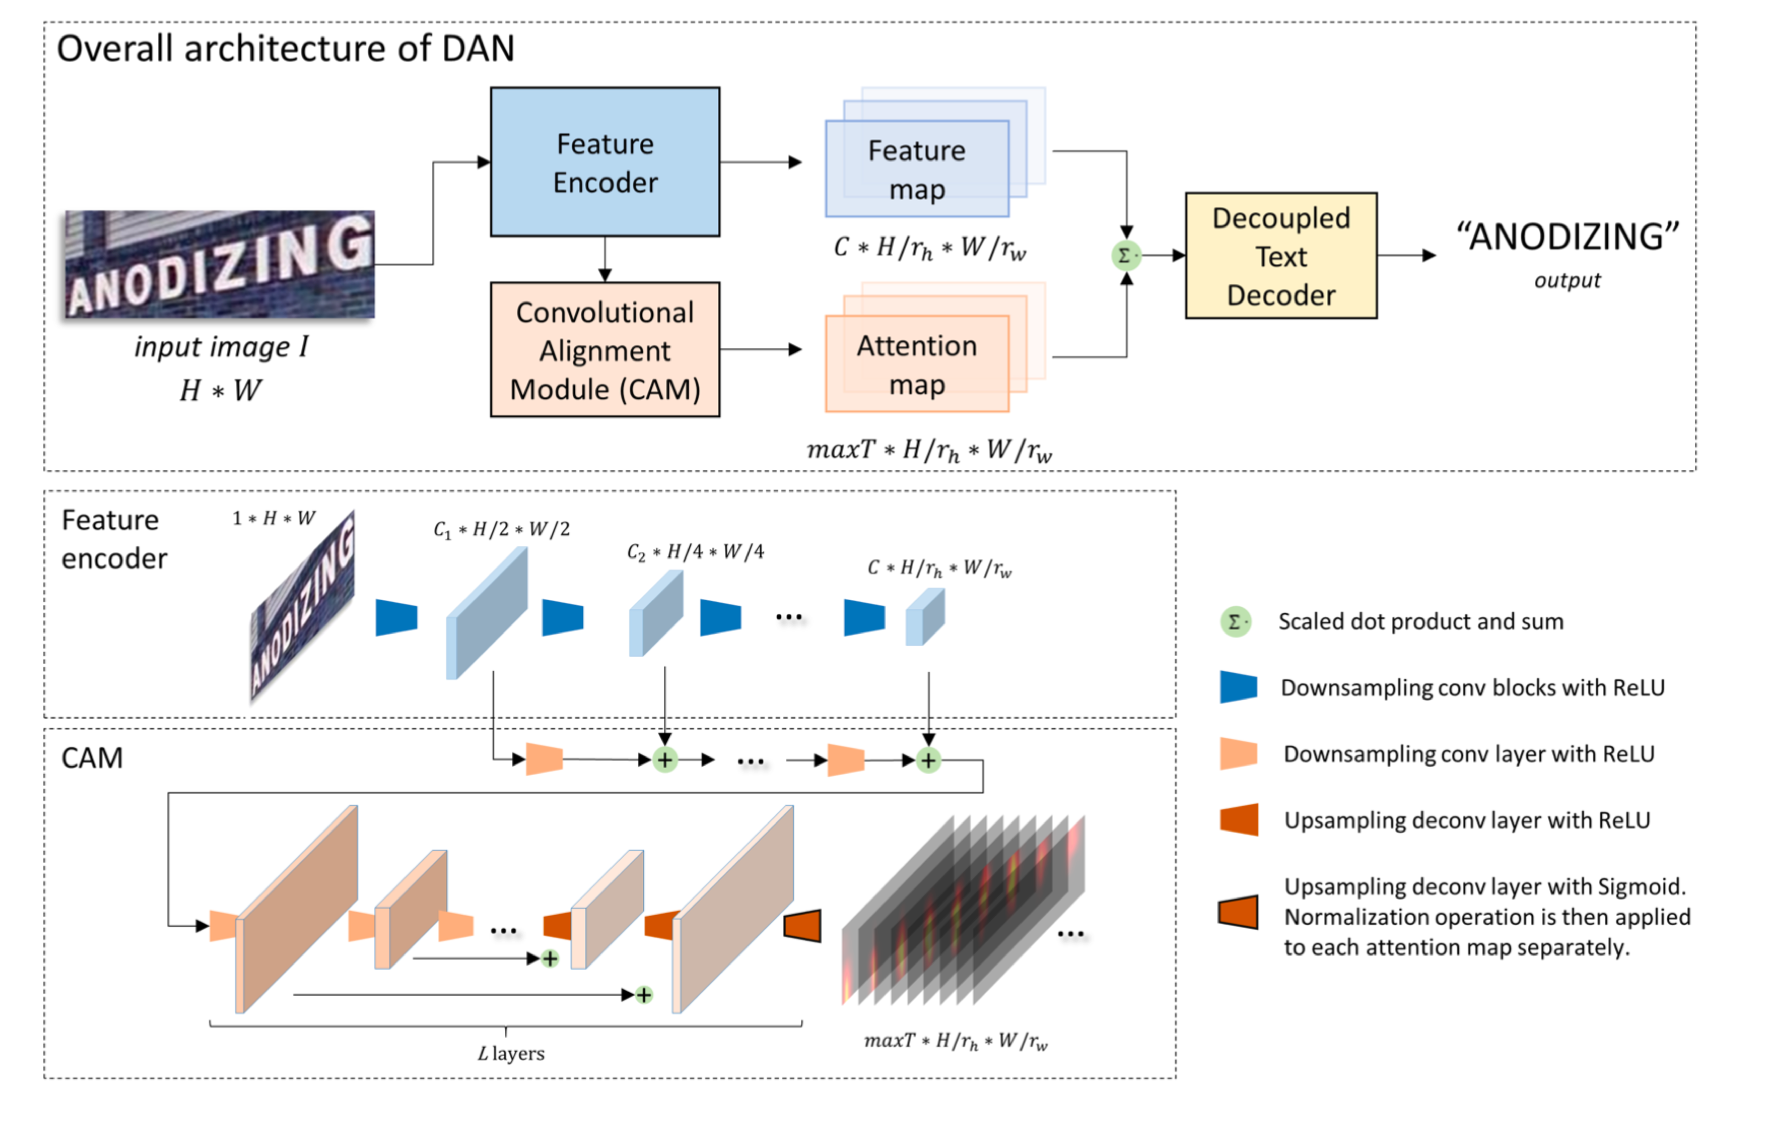
\includegraphics[width=.9\textwidth]{figure/recognition/dan_framework.png} 
    \caption{DAN网络结构。} 
    \label{dan_framework} 
\end{figure}

\subsection{GTC (AAAI2020)}
GTC\cite{hu2020gtc}的主要是解决基于CTC的文字识别器中帧数不对齐的问题,比如字符'H'由于分帧的原因会被识别为'I'。
文章中通过基于注意力机制的识别head的监督来使得特征在一定程度上对齐。在测试阶段为了保证效率,只使用基于CTC的识别head。
另外,CNN特征经过分帧后,相邻帧之间在视觉上具有一定的相似性,为了使得特征能够进一步对齐(理想情况下一帧的特征代表一个字符的特征),
作者使用GCN来建模帧之间的关系,融合后得到对齐的帧。
\begin{figure}[H]
    \centering
    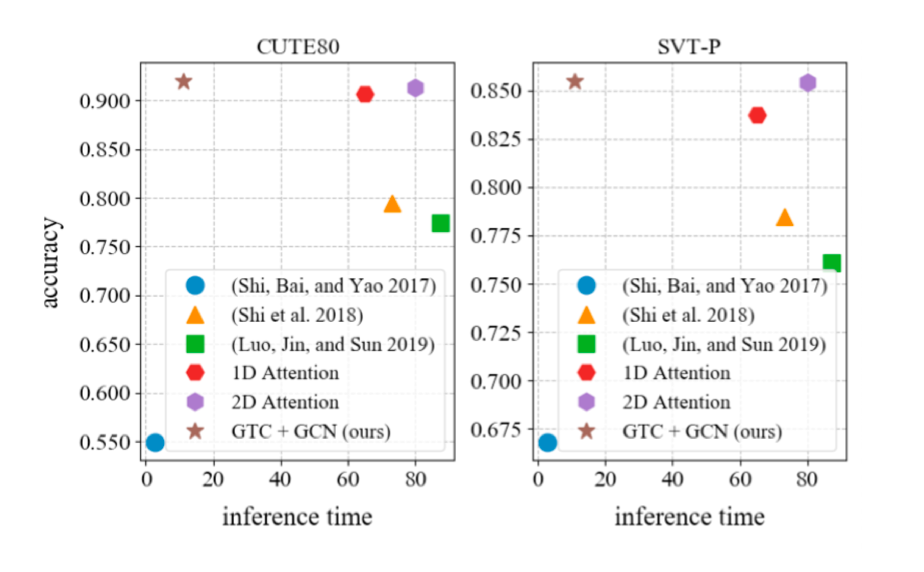
\includegraphics[width=.8\textwidth]{figure/recognition/gtc_introduction.png} 
    \caption{GTC准确率和效率的关系,x轴代表ms/image} 
    \label{gtc_introduction} 
\end{figure}

\subsubsection{GTC的网络结构}
GTC的网络结构如图\ref{gtc_framework}所示:网络的整体结构和Aster类似,不同的是,识别的head是基于CTC的,基于注意力机制的识别head在训练时
起到辅助作用,使得特征能够起到一定的对齐作用。为保证效率,测试过程只使用CTC进行解码,最终的精度-效率对比如图\ref{gtc_introduction}所示。
\begin{figure}[H]
    \centering
    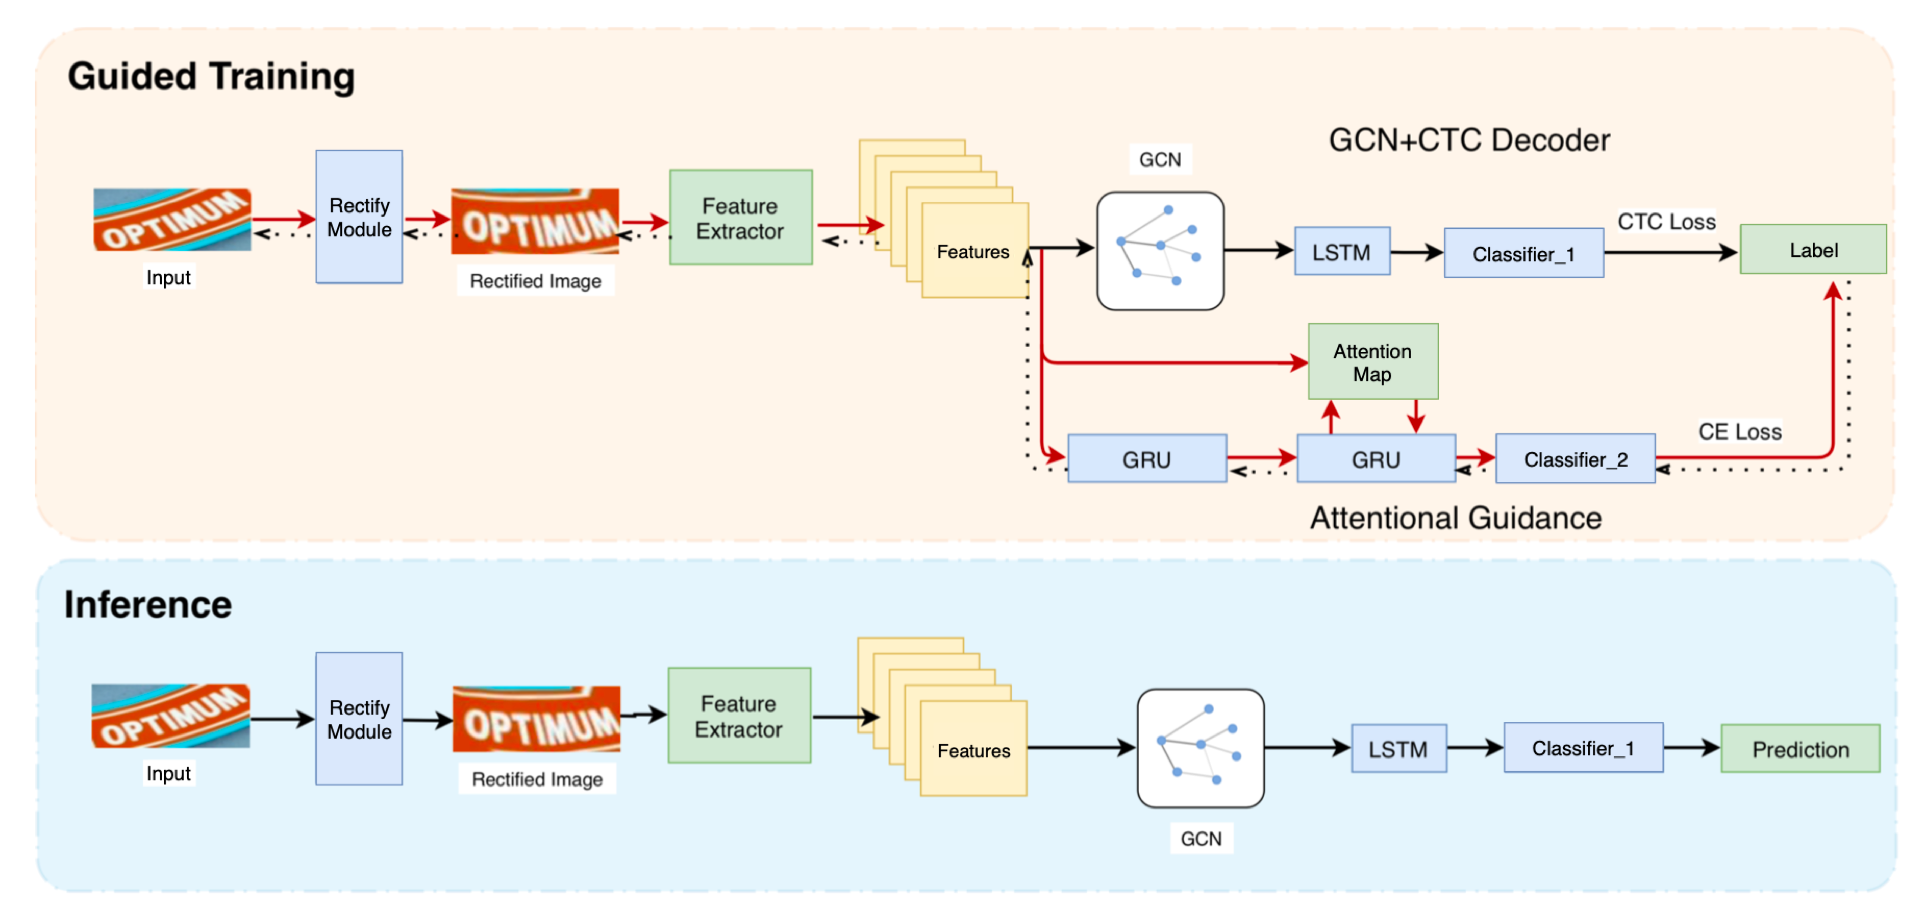
\includegraphics[width=.98\textwidth]{figure/recognition/gtc_framework.png} 
    \caption{GTC网络结构。} 
    \label{gtc_framework} 
\end{figure}


\subsection{TextScanner (AAAI2020)}
TextScanner\cite{wan2019textscanner}的主要是解决基于分割的文本识别器中字符分割不准以及基于注意力机制的文本识别器中注意力发散的问题。目的仍然是
寻找精准的字符定位从而使得特征对齐。如图\ref{textscanner_introduction}:基于注意力机制和分割的方法对字符的定位都存在一些问题,文章中通过预测单词
的阅读顺序来解决该问题。

\begin{figure}[H]
    \centering
    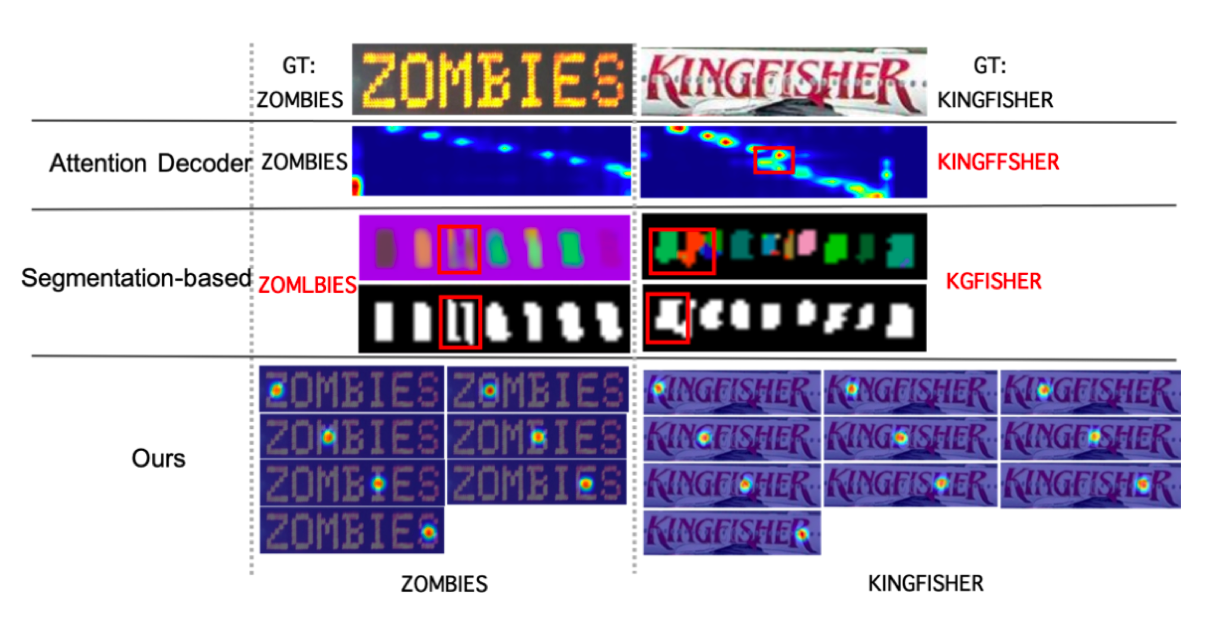
\includegraphics[width=.8\textwidth]{figure/recognition/textscanner_introduction.png} 
    \caption{TextScanner问题出发点:Attention Decoder中注意力容易发散;基于分割的方法中因为阈值问题,容易存在欠分割或过分割问题。} 
    \label{textscanner_introduction} 
\end{figure}

\subsubsection{TextScanner的网络结构}
TextScanner的网络结构如图\ref{scatter_framework}所示:整体分为三部分,1)字符分割模块,每个像素对类别进行预测;2)字符顺序分割模块,其中N代表
最大长度,模块进行N分类,预测每个像素属于哪一时间时刻;3)字符定位模块用于定位每个字符。
\begin{figure}[H]
    \centering
    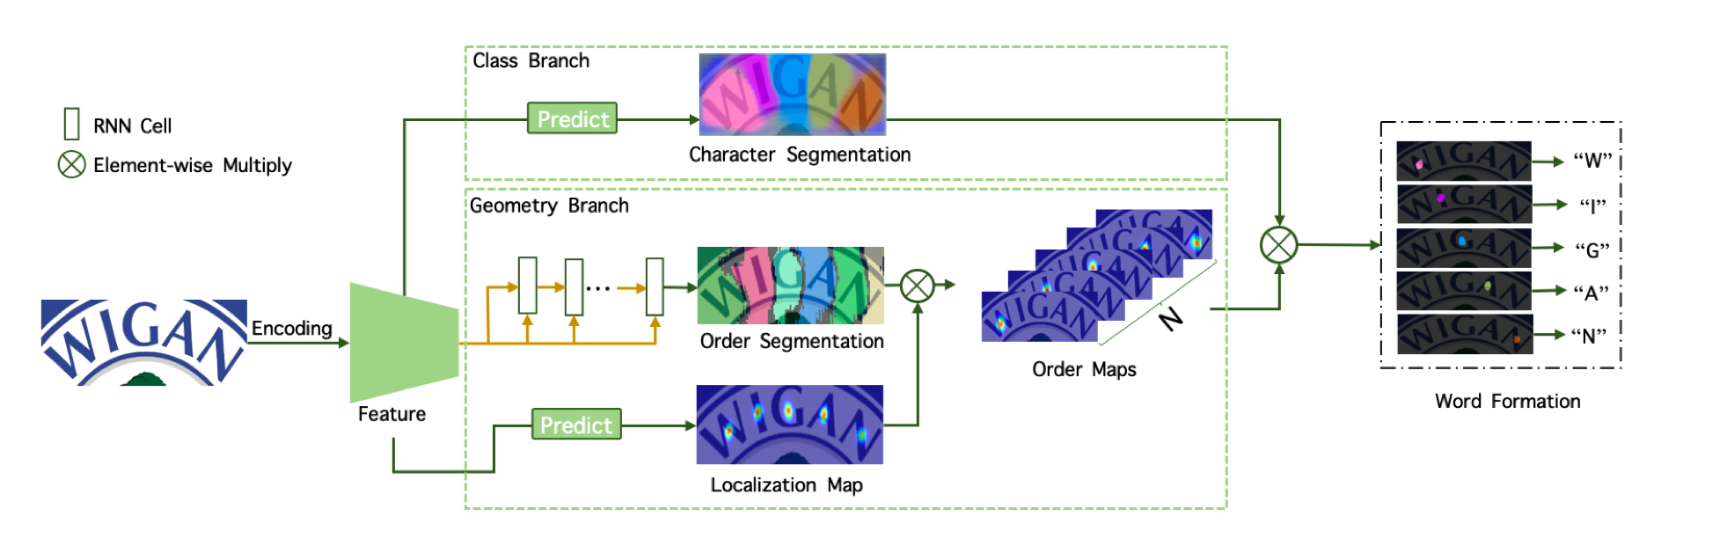
\includegraphics[width=.98\textwidth]{figure/recognition/textscanner_framework.png} 
    \caption{TextScanner网络结构。} 
    \label{textscanner_framework} 
\end{figure}

\subsection{SCATTER (CVPR2020)}
SCATTER\cite{scatter}的主要研究目的是让网络不断迭代地选择图像的视觉特征(CNN的特征)和语义特征(RNN建模出的语义特征)来强化
模型的特征提取能力。而特征选择的过程通过注意力机制来完成。
\subsubsection{SCATTER的网络结构}
SCATTER的网络结构如图\ref{scatter_framework}所示,网络的整体框架和Aster一致,不同之处在于:SCATTER在Visual features
和Contextual features之间加入了多层特征选择模块进行特征的优化,并且在Visual features中加入了CTC进行监督学习。特征选择模块
网络结构如图\ref{scatter_feature_select}所示。
\begin{figure}[H]
    \centering
    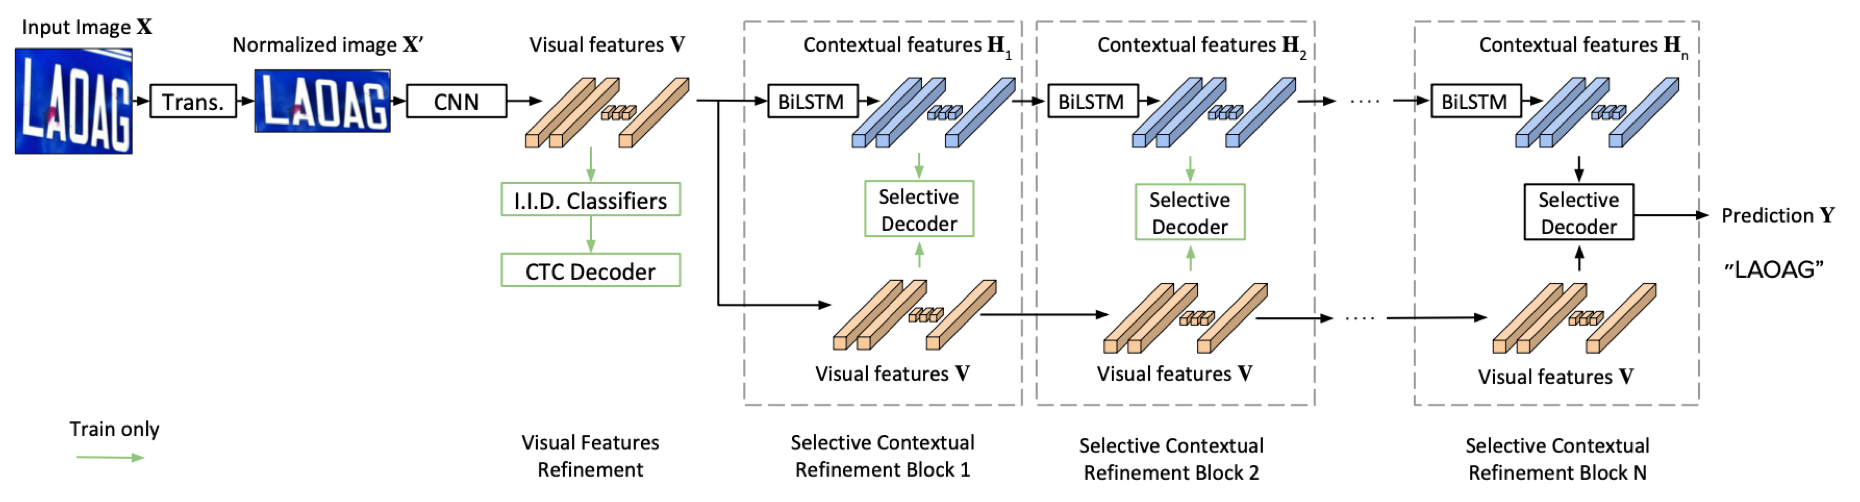
\includegraphics[width=.98\textwidth]{figure/recognition/scatter_framework.png} 
    \caption{SCATTER网络结构。} 
    \label{scatter_framework} 
\end{figure}

\begin{figure}[H]
    \centering
    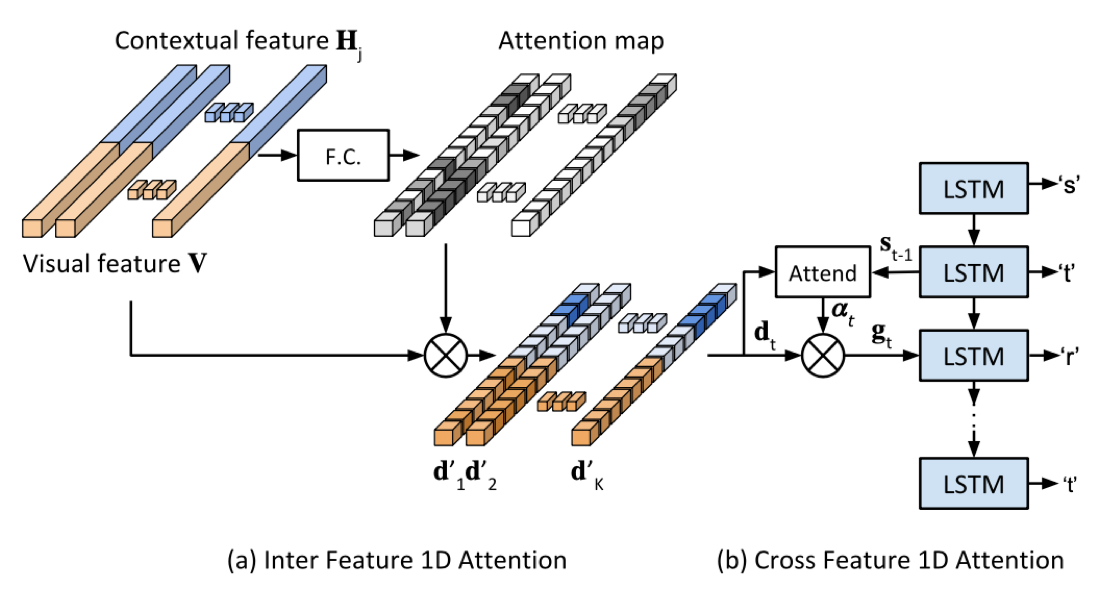
\includegraphics[width=.8\textwidth]{figure/recognition/scatter_feature_select.png} 
    \caption{SCATTER特征选择模块。} 
    \label{scatter_feature_select} 
\end{figure}

\subsection{SRN (CVPR2020)}
SRN\cite{2020srn}的主要出发点是:
1)在文字识别中,由于光照,旋转等因素的影响,仅仅依靠图像的视觉特征
极易引起单词中某个字符预测错误。对于这些易错的字符,如果能够利用单词的语义信息,那么
将会极大地降低该字符的预测错误率。如图\ref{srn_introduction}所示,如果仅仅观察每个字符的视觉特征(b),
某些字符容易预测错误,结合上下文语义信息能够缓解因视觉特征混淆而引起的错误预测。
2)文字识别中基于注意力机制的识别器中\cite{shi2018aster},注意力模块的输出大多是串行的,注意力模块中当前时刻
的预测非常依赖于前一时刻的输出,导致模型难以并行处理。为解决模型的效率问题,提出并行的注意力模块。


\begin{figure}[H]
    \centering
    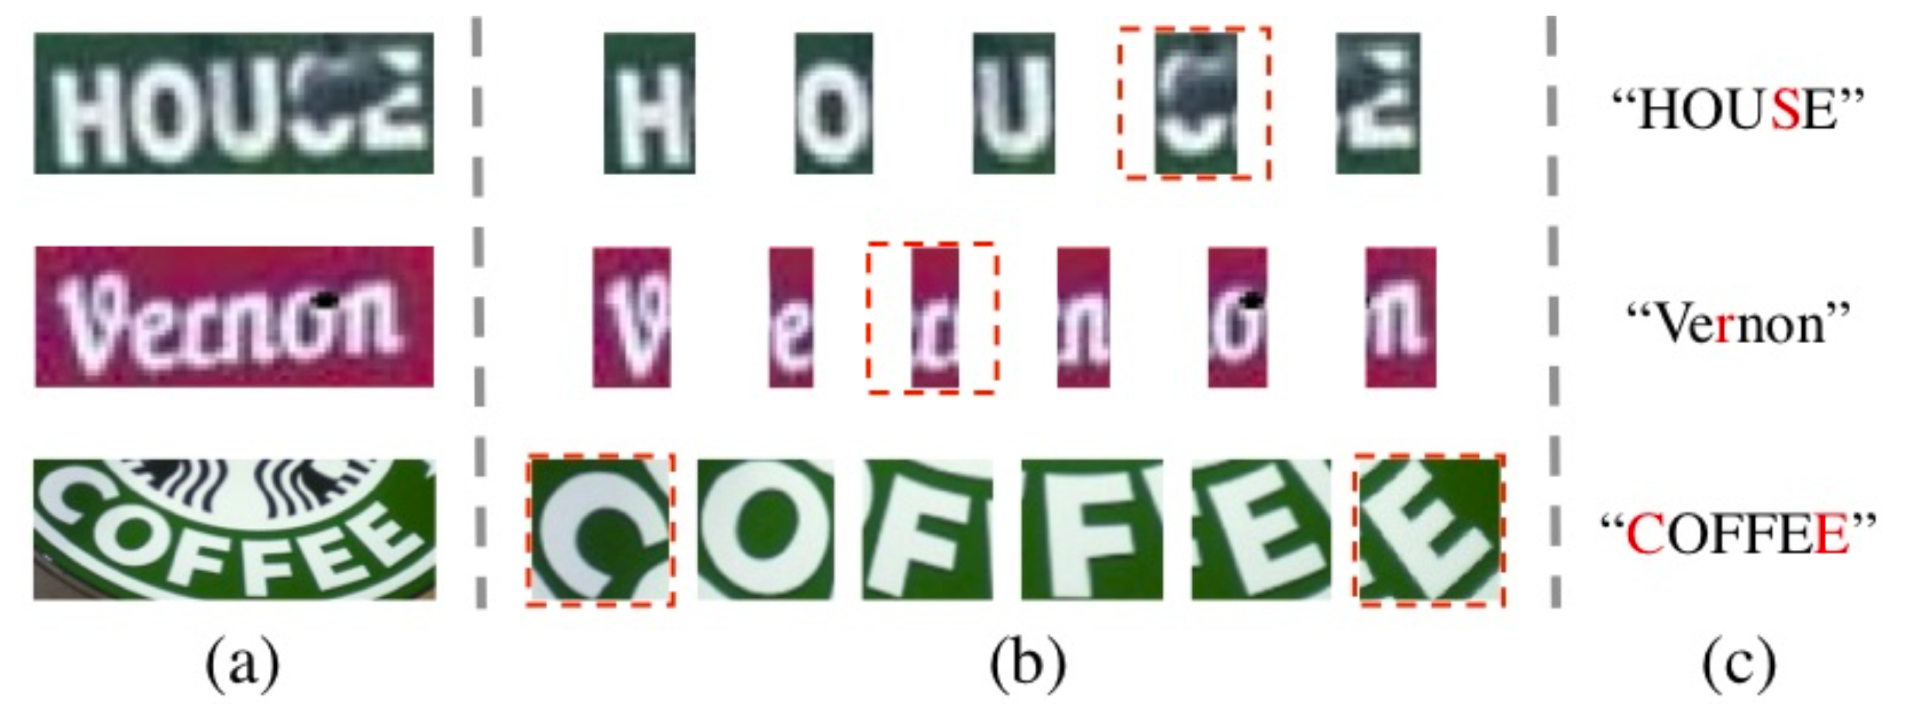
\includegraphics[width=.7\textwidth]{figure/recognition/srn_introduction.png} 
    \caption{单词中容易预测错误的字符案例:(a)表示原图;(b)表示字符,红色标注为易错字符;(c)为利用上下文语义信息预测结果。} 
    \label{srn_introduction} 
\end{figure}

\subsubsection{SRN的网络结构}
SRN的网络结构如图\ref{srn_framework}所示:1)整体网络的backbone为FPN网络,用于提取图像的视觉特征;2)并行的视觉注意力模块(PAVM)用于定位每个字符;3)全局的语义推理模块(GSRM)
用于利用语义上下文来预测字符。
\begin{figure}[H]
    \centering
    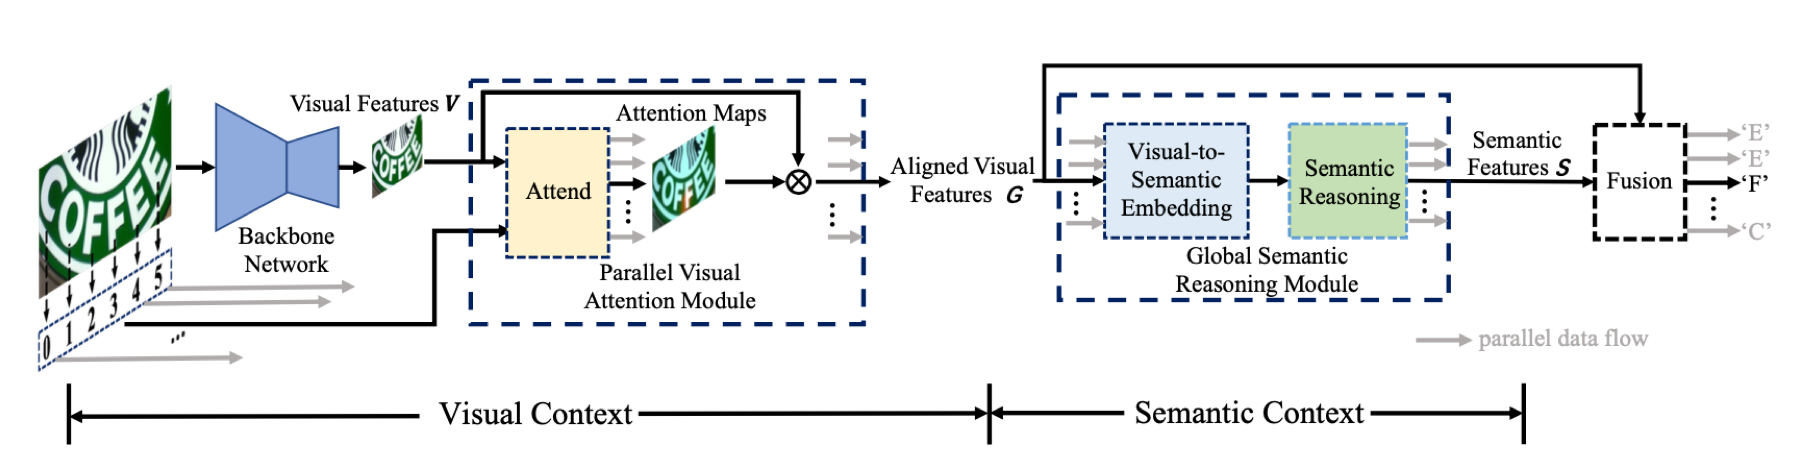
\includegraphics[width=.98\textwidth]{figure/recognition/srn_framework.png} 
    \caption{SRN网络框架图。} 
    \label{srn_framework} 
\end{figure}

\begin{figure}[H]
    \centering
    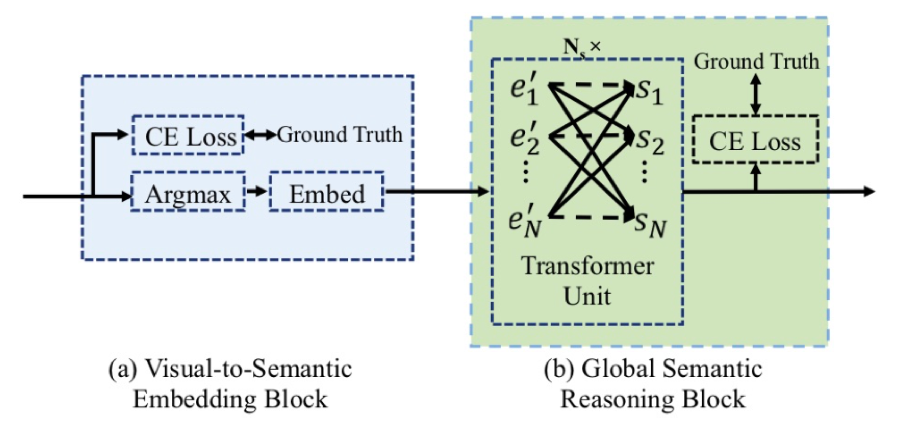
\includegraphics[width=.7\textwidth]{figure/recognition/srn_gsrm.png} 
    \caption{GSRM模块结构。} 
    \label{srn_gsrm} 
\end{figure}
\subsubsection{SRN并行以及语义推理分析}
SRN的主要优势在于利用单词的上下语义来预测困难字符,而要实现这一特性的技术难点却在于如何并行化处理序列预测。
因为在预测t时刻的字符时,需要其他所有时刻的特征。因此,SRN中如何将各个模块并行化是该方法技术的重点。
表\ref{srn_process}详细地对比了SRN中并行化与Aster中串行化的区别。

对于并行化处理方面,SRN的主要改进在于两大方面:1)将注意力模型并行化。传统的注意力模型
依赖于前一时刻的隐藏状态$h_{t-1}$(在注意力模块中,$h_{t-1}$作为key来获取相似度)从而无法并行化。SRN中将
传统注意力模型中的key改为$O_{t}$(代表字符顺序,第一个字符为0,第二个字符为1)的Embedding特征,从而实现并行化;
2)将语义模型并行化。先前的文字识别算法中利用rnn来对文字语义进行建模,而rnn中以前一时刻的预测结果的Embedding特征
$f_{y}(y_{t-1})$作为输入,从而无法并行化。SRN中将$e_{t}^{'}$(以$g_{t}$为输入的预测结果的Embedding向量)来代替,
从而实现并行化。另外,通过Transformer Unit来获取多路径的语义信息,能够考虑当前时刻的前向以及后向的所有语义信息。
\begin{table}[!htbp]
    \centering
    \caption{SRN中PVAM,GSRM模块和Aster的串行注意力机制与串行语义模块的区别。其中TU为Transformer Unit,
    $v_{i}$为视觉特征,$h_{i}$为隐藏状态,$y_{t}$为字符label,$O_{t}$为阅读顺序。} 
    \begin{tabular}{|c|l|l|}
    \hline 
    Module&Aster&SRN\\
    \hline 
    \multirow{3}*{Attention}&
    $e_{t,i}=W^{T}_{e}tanh(W_{h}h_{t-1} + W_{v}v_{i})$& 
    $e_{t,i}=W^{T}_{e}tanh(W_{o}f_{o}(O_{t}) + W_{v}v_{i})$\\
    &$\alpha_{t,i}=exp(e_{t,i})/\sum_{i^{'}=1}^{n}exp(e_{t,i^{'}})$&
    $\alpha_{t,i}=exp(e_{t,i})/\sum_{i^{'}=1}^{n}exp(e_{t,i^{'}})$\\
    &$g_{t}=\sum_{i=1}^{n}\alpha_{t,i}v_{i}$&
    $g_{t}=\sum_{i=1}^{n}\alpha_{t,i}v_{i}$\\
    \hline 
    \multirow{2}*{Semantic Reasoning}&
    \multirow{2}*{$(x_{t}, h_{t}) = rnn(h_{t-1}, (g_{t}, f_{y}(y_{t-1})))$}&
    $e_{t}^{'} = f_{e}(softmax(f_{g}(g_{t})))$\\
    &&$s_{t} = TU(e_{0}^{'}...e_{t-1}^{'}e_{t+1}^{'}...e_{n}^{'})$\\
    \hline 
    \multirow{2}*{Fusion}&&$z_{t} = sigmoid(W_{z}[g_{t},s_{t}])$\\
    &&$f_{t} = z_{t}g_{t} + (1-z_{t})s_{t}$\\
    \hline 
    Classification&
    $p(y_{t}) = softmax(Wx_{t}+b)$&
    $p(y_{t}) = softmax(Wf_{t}+b)$\\
    \hline
    \end{tabular}
    \label{srn_process} 
\end{table}

\begin{figure}[H]
    \centering
    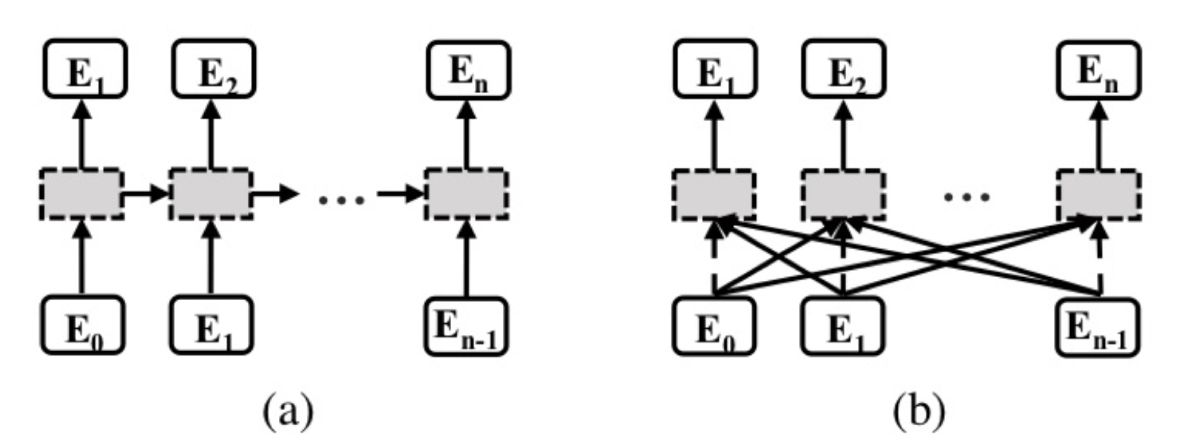
\includegraphics[width=.8\textwidth]{figure/recognition/srn_multiway.png} 
    \caption{a)rnn中建模单词语义模型;b)SRN中建模单词语义模型能够考虑各个路径的信息,避免单向的错误累积。} 
    \label{srn_multiway} 
\end{figure}

% \subsection{SEED (CVPR2020)}
% Not Publication